\chapter{Manuel d'utilisation}

L'interface de l'éditeur est assez intuitive. Les boutons sont peu nombreux et les fonctionnalités moins utilisées sont dans la barre de menu.
Ce manuel liste la totalité des fonctionnalités du logiciel.

\section{Interaction}

\subsection{Barre de menu}


Les actions disponibles dans la barre de menu sont les suivantes :
\begin{itemize}
\item \emph{File...} : Ouvrir / Sauvegarder / Fermer
\item \emph{Edit...} : Indenter
\item \emph{Schéma...}
	\begin{itemize}
	\item \emph{Load schema file} : Ouvre un schéma et le lie automatiquement au fichier XML.
	\item \emph{Generate schema file} : Génère automatiquement un schéma à partir du fichier XML en utilisant les balises connues.
	\item \emph{Delete schema} : Supprime la liaison entre le schéma et le fichier XML.
	\end{itemize}
\end{itemize}

\paragraph{}
Les actions Ouvrir, sauvegarder, indenter et valider sont disponibles en accès rapide sur la barre des boutons.

\subsection{Raccourcis}
\begin{itemize}
\item \emph{ctrl + o} : Ouvrir
\item \emph{ctrl + r} : Lancer la validation
\item \emph{ctrl + s} : Enregistrer 
\item \emph{ctrl + shift + s} : Enregistrer sous
\item \emph{ctrl + i} : Indenter automatiquement les lignes sélectionnées
\item \emph{F4} : Switch entre le fichier XML et le schéma
\end{itemize}

\section{Validation}
La validation permet de vérifier si le code XML entré est valide.
Il vérifie que les balises sont correctement formés (pas de balises croisés).
Et si un schéma est associé, le validateur vérifie que le fichier XML est bien en accord avec celui-ci.
En cas d'erreur, le message d'erreur est indiqué dans la console et le numéro de la ligne concernée est surligné en rouge.
Si la validation s'exécute correctement, la vue arborescence est générée.

\section{Vue arborescente}
Sur la vue arborescence il est possible de renommer un noeud (double clic), supprimer un noeud (clic droit / Supprimer), ou déplacer un noeud (glisser/déposer).
Lors d'une modification, la vue de l'éditeur de texte est automatiquement mise à jour.

\section{A propos du schéma}
L'association d'un schéma est une option du logiciel mais il n'est pas obligatoire de lier un schéma pour travailler un fichier XML.
Quand un schéma est ouvert, il est "lié" au fichier XML. La balise de lien vers le schéma est automatiquement ajoutée dans le fichier XML
et un enregistrement provoque la sauvegarde des deux fichiers (xml et schéma).
Lors de l'ouverture d'un fichier XML, le schéma est automatiquement ouvert si un chemin vers celui-ci est indiqué dans le XML.

\section{Fonctions du logiciel}


\begin{figure}[h!]
\noindent\makebox[\textwidth]{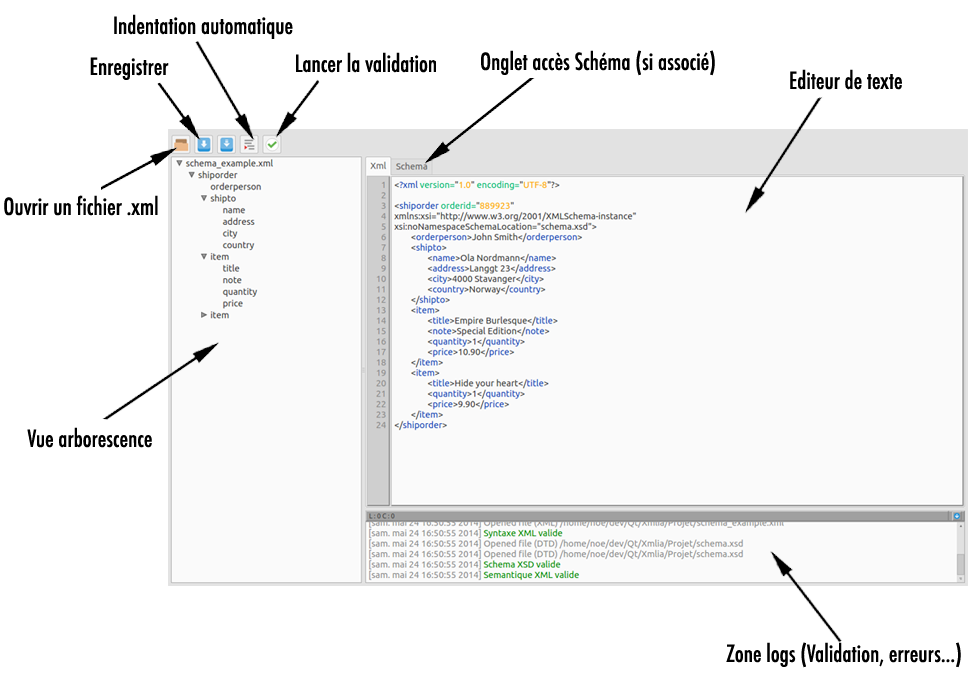
\includegraphics[width=450pt]{images/help1.png}}
\caption{Différentes sections du logiciel}
\end{figure}
